\subsubsection{Trends in Independent Features}\label{sec:impl-data-analysis:independent-features}
The feature transformation based on collinearity factor carried out in the Section \ref{sec:impl-data-analysis:corr:generic-approach} has reduced the number of features present in the dataset to 33. The new overall feature correlation statistics have been illustrated in Figure \ref{fig:corr:post-transformation}. From same, a number of independent features, where correlation factor is close to 0, can be observed.

The first candidate for trend analysis is illustrated in Figure \ref{fig:corr:post-transformation:overallCoverage-complaxity-ncloc} and consisted of \overallCoverage{}, \complexity{} and\ncloc{} features. It should be noted that while \ncloc{} and \complexity{} attributes display a strong positive correlation the \overallCoverage{} feature is unrelated to either of the two attributes. Same observation can be made from Figure \ref{fig:corr:post-transformation:overallCoverage-complaxity-ncloc} where the metric representing the number of source code lines, \ncloc{}, and the metric representing overall complexity of the code move together. Additionally, despite lack of strong indication of the collinearity, the overall coverage metric increases in value along the source code line metric. Taking into the account the domain knowledge of any software development project, the greater the number of the source code lines present the larger the number of code to be covered by a test automation. What is interesting in the underlying scenario is that the growth of source code is closely followed by the increase of test automation coverage. 

\begin{figure}[!h]
    \centering
    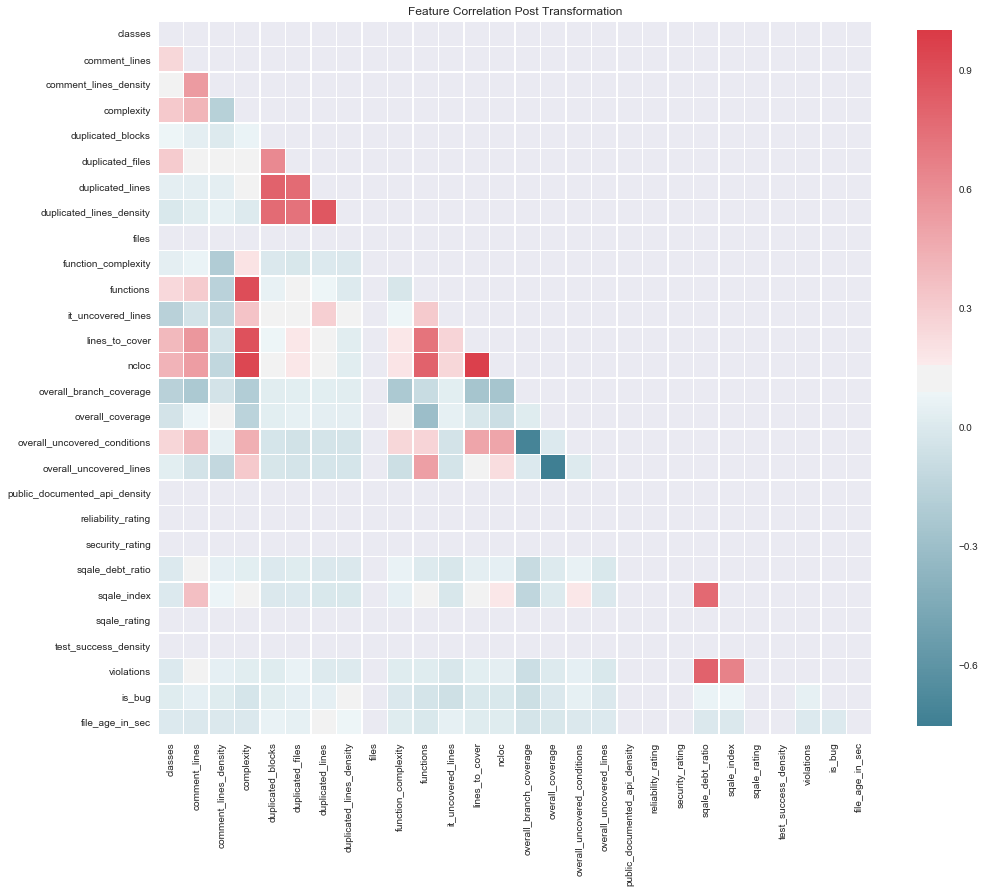
\includegraphics[scale=0.5]{Figures/correlation/Feature_Correlation_Post_Transformation.png}
    \caption{Feature Correlation after Feature Transformation}
    \label{fig:corr:post-transformation}
\end{figure}

\begin{figure}
    \centering
    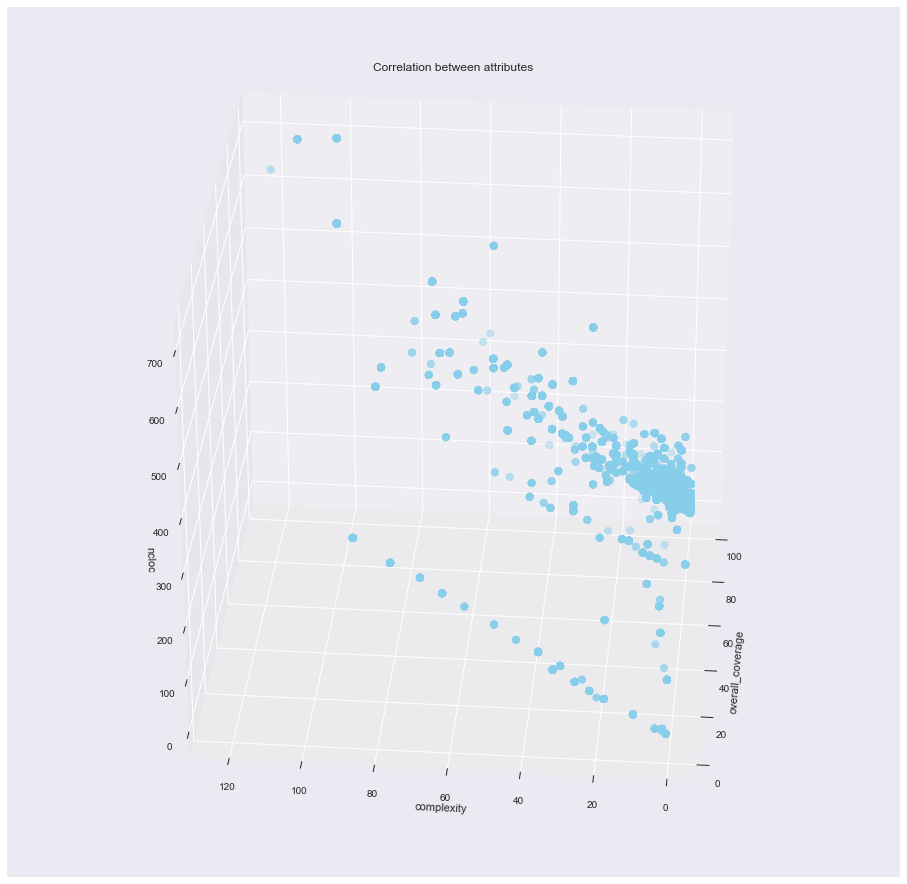
\includegraphics[scale=0.5]{Figures/independent-feat-trends/Correlation_between_attributes_overall_coverage_complexity_ncloc.png}
    \caption{Independent Features Correlation - \overallCoverage{}, \complexity{} and \ncloc{}}
    \label{fig:corr:post-transformation:overallCoverage-complaxity-ncloc}
\end{figure}

\begin{figure}
    \centering
    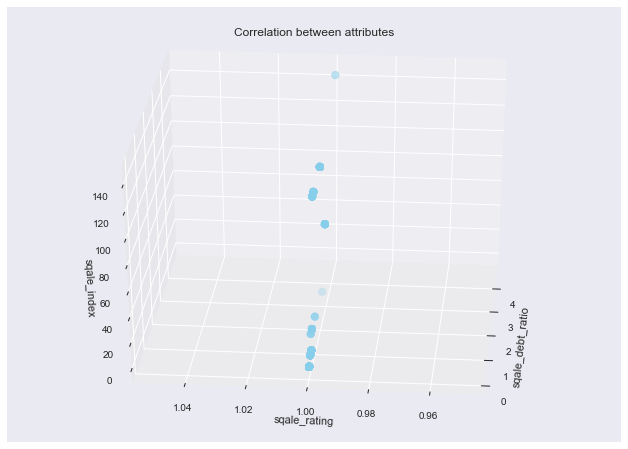
\includegraphics[scale=0.7]{Figures/independent-feat-trends/Correlation_between_attributes_sqale_debt_ratio_sqale_rating_sqale_index.png}
    \caption{Independent Features Correlation - SQALE Metrics}
    \label{fig:corr:post-transformation:sqale}
\end{figure}
\FloatBarrier